\chapter{勒贝格测度}

本章主要讨论~$\R$~中点集的测度理论, 先以第一章的``开集构造定理''为基础定义
一维有界开集、闭集的测度, 然后利用它们定义出~$\R$~中一般有界集的外测度与内测度,
进而给出~$\R$~中可测集的定义并讨论其性质. 另外, 简要介绍了~$\R^n$~中点集测度、波雷尔集以及不可测集的存在性.

回顾序章中介绍的勒贝格积分的大体思路, $f(x)$~在~$[a,\, b]$~上的勒贝格积分可定义为
\begin{equation} \label{eq20}
(L)\int_a ^b \!\! f(x) \mathrm{d}x = \lim_{\lambda \to 0} \sum^n _{i=1} \xi_i |E_i|
\end{equation}
其中, $\xi_i \in [y_{i-1},\,y_i]$
\[
E_i = \big\{ x \in [a,\,b]: \: y_{i-1} \leqslant f(x) < y_i \big\}
\]
$|E_i|$~表示一维集合~$E_i$~的``长度''.

可见, 建立勒贝格积分理论不可避免地要对~$\R^n$~中的一般点集给出类似于
一维区间长度的``适当的度量'', 为了测量~$\R^n$~中一般的集合的``大小''引入一种
适当的度量\raisebox{0.5mm}{-----}测度\index{测度}, 用~$m(\cdot)$~表示. 这种测度是长度、面积、
体积的推广, 并且要满足下列性质(以一维为例):

(i) (\textbf{非负性}) $m(E) \geqslant 0;$

(ii) (\textbf{有限可加性}) 若~$E_1 \cap E_2 = \emptyset$, 则
\[
m(E_1 \cup E_2) = m(E_1)+m(E_2)
\]

(iii) (\textbf{正则性}) $m\big([0,\,1]\big) = 1$.

以上三条性质又称为勒贝格测度公理.

\section{一维有界开集、闭集的测度}

\subsection{一维有界开集、闭集测度的定义}

\begin{definition}
设~$G \subset \R$~为有界开集, 由开集构造定理, $G = \smallcup\limits_k
(\alpha_k,\,\beta_k)$ ($k$~有限或可列, $(\alpha_k,\,\beta_k)$~为~$G$~的构成区间,
互不相交), 则
\[
m(G) = \sum_k (\beta_k - \alpha_k)
\]
称为一维有界开集~$G$~的测度\index{开集测度}.
\end{definition}

\begin{remark}
该定义要求~$m(G) < +\infty$, 即级数~$\sum\limits_{k=1}^\infty (\beta_k - \alpha_k)$~收敛.
$G$~有界, 则存在~$a,\,b \in \R$~使得~$G \subset (a,\,b)$.
又~$(\alpha_k,\,\beta_k)$~互不相交, 故对~$\forall~n \in \N$
\[
\sum^n _{k=1} (\beta_k - \alpha_k) \leqslant b-a
\]
令~$n \rightarrow \infty$, 得
\[
\sum^\infty_{k=1} (\beta_k - \alpha_k) \leqslant b-a < +\infty
\]
\end{remark}

\begin{definition}
设~$F \subset \R$~为有界闭集, 任取开区间~$(a,\,b) \supset F$,
令~$G = (a,\,b) - F$, 则~$G$~为~$\R$~中的有界开集
\[
m(F) = b - a - m(G)
\]
称为一维有界闭集~$F$~的测度\index{闭集测度}.
\end{definition}

\begin{remark}
(i) 对~$\forall~(a,\,b) \supset F$~都有~$m\big((a,\,b)-F\big) = b - a - m(F)$;

(ii) 上述定义中~$F$~的测度与开区间的选取无关;

(iii) $m\big( [a,\,b] \big) = b - a$.
\end{remark}

\begin{proof}
(i) 显然.

(ii) 若~$F$~为单点集. 设~$F = \{x\},\,x \in (a,\,b)$, 则~$G = (a,\,b) - \{x\}
= (a,\,x) \cup (x,\,b)$. 从而
\[
m(F) = b - a - m(G) = b -a -[(x-a)+(b-x)] = 0
\]

若~$F$~不是单点集. 令
\[
\alpha = \inf\{x: \: x\in F\},\quad \beta = \sup\{x: \: x\in F\}
\]
则~$\alpha \neq \beta$~且~$\alpha,\,\beta \in F$. 设~$F \subset (a,\,b),\,
G = (a,\,b) - F$, 则
\[
G = (a,\,\alpha) \cup (\beta,\,b) \cup \big( (\alpha,\,\beta) - F \big)
\]

\begin{figure}[!h]
\centering
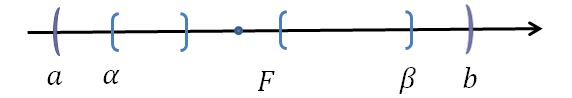
\includegraphics[width=0.5\textwidth]{image/ClosedSet.jpg}
\end{figure}

\noindent 故~$m(G) = \alpha - a + b - \beta + m\big( (\alpha,\,\beta) - F \big)$, 从而
\[
m(F) = b-a - m(G) = \beta - \alpha - m\big( (\alpha,\,\beta) - F \big)
\]

(iii) 由~(ii)~的证明知, $m\big([a,\,b]\big) = b - a - m\big( (a,\,b)
- [a,\,b] \big) = b - a$.
\end{proof}

\medskip

\begin{example}
求康托尔集的测度.
\end{example}

\medskip

\begin{solution}
记挖去的开区间全体为~$G_0$, 则~$G_0$~是~$\R$~中的有界开集, 故
\[
m(G_0) = \frac{1}{3} + \frac{2}{3^2} + \cdots + \frac{2^n}{3^{n+1}} + \cdots = 1
\]
从而~$m(C) = m\big([0,\,1]\big) - m(G_0) = 0$. 因此, 康托尔集是测度为~$0$~的不可列集.
\end{solution}

\subsection{一维有界开集测度的性质}

\begin{proposition} \label{prop221}
$\R$~中的有界开集测度具有如下性质:

(i) (\textbf{非负性}) $m(G) \geqslant 0$;

(ii) (\textbf{单调性}) 若~$G_1 \subset G_2$, 则~$m(G_1) \leqslant m(G_2)$;

(iii) (\textbf{次可加性}\index{次可加性}) 设~$k$~有限或可列
\[
m\big( \medcup_k G_k \big) \leqslant \sum_k m(G_k)
\]
\noindent 若~$G_k$~互不相交, 则
\[
m\big( \medcup_k G_k \big) = \sum_k m(G_k)
\]
\end{proposition}

\begin{proof}
(i) 显然.

(ii) 设~$G_1 = \smallcup\limits_k \big(\alpha^{(1)}_k,\,\beta^{(1)}_k\big),\,
G_2 = \smallcup\limits_k \big(\alpha^{(2)}_k,\,\beta^{(2)}_k \big)$, 则
\[
m(G_1) = \sum_k \big(\beta^{(1)}_k - \alpha^{(1)}_k\big), \quad m(G_2) =
\sum_k \big(\beta^{(2)}_k - \alpha^{(2)}_k\big)
\]
故对~$\forall~\varepsilon > 0$, 存在~$n_0 \in \N$~使得
\[
m(G_1) < \sum^{n_0}_{k=1} \big(\beta^{(1)}_k - \alpha^{(1)}_k\big) + \varepsilon
\]
由于~$G_1 \subset G_2$, 由命题~\ref{prop151}, $\big(\beta^{(1)}_k -
\alpha^{(1)}_k\big),\,k=1,\,\cdots,n_0$~必含于某~$m_0$~个~$G_2$~的构成区间
~$\big(\alpha^{(2)}_{k_j},\,\beta^{(2)}_{k_j} \big), j=1,\,\cdots,\,m_0$~
中($m_0 \leqslant n_0$), 故
\[
\sum^{n_0}_{k=1} \big(\beta^{(1)}_k - \alpha^{(1)}_k\big) \leqslant \sum^{m_0}_{j=1}
\big(\beta^{(2)}_{k_j} - \alpha^{(2)}_{k_j} \big)
\]
从而
\[
m(G_1) < \sum^{m_0}_{j=1} \big(\beta^{(2)}_{k_j} - \alpha^{(2)}_{k_j} \big) + \varepsilon \leqslant m(G_2) + \varepsilon
\]
由~$\varepsilon$~的任意性, $m(G_1) \leqslant m(G_2)$.

(iii) 不妨设~$\sum\limits_k m(G_k)<+\infty$, 否则显然成立.
记~$G = \smallcup\limits_k G_k$~是开集, 设
\[
G_k = \medcup\limits_i \big(\alpha^{(k)}_i,\, \beta^{(k)}_i \big),\quad
G = \medcup_j (\alpha_j, \, \beta_j)
\]
则每个区间~$(\alpha_j, \, \beta_j)$~都是某些小区间~$\big(\alpha^{(k)}_i,\,
\beta^{(k)}_i \big)$~的并. 由于~$\big\{(\alpha_j, \, \beta_j)\big\}$~互不相交,
故当~$j$~不同时, 构成~$(\alpha_j,\,\beta_j)$~的小区间的并也互不相交.
于是, 对任意的~$0 < \varepsilon < (\beta_j - \alpha_j)/2$,
闭区间~$[\alpha_j+\varepsilon,\,\beta_j -\varepsilon]$~中每个点都是构成
~$(\alpha_j,\,\beta_j)$~的某个小区间~$\big(\alpha^{(k)}_i,\, \beta^{(k)}_i \big)$~的
内点, 即~$[\alpha_j+\varepsilon,\,\beta_j -\varepsilon]$~中每个点都被
某个小开区间~$\big(\alpha^{(k)}_i,\, \beta^{(k)}_i \big)$~覆盖. 由有限开覆盖定理,
这些小区间~$\big(\alpha^{(k)}_i,\, \beta^{(k)}_i \big)$~中的有限个小开区间就可以
覆盖~$[\alpha_j+\varepsilon,\,\beta_j -\varepsilon]$, 故
\begin{eqnarray*}
\beta_j - \alpha_j - 2 \varepsilon &\leqslant& m\Big( \mbox{有限个~}
\big(\alpha^{(k)}_i,\, \beta^{(k)}_i \big) \Big) \\
&\leqslant& m \Big( \mbox{构成~}(\alpha_j, \, \beta_j)\mbox{~的所有~}
\big(\alpha^{(k)}_i,\, \beta^{(k)}_i \big) \Big)
\end{eqnarray*}
令~$\varepsilon \to 0$, 得
\[
\beta_j - \alpha_j \leqslant m \Big( \mbox{构成~}(\alpha_j, \, \beta_j)\mbox{~的所有~}
\big(\alpha^{(k)}_i,\, \beta^{(k)}_i \big) \Big)
\]
从而对所有的~$j$~求和得到
\begin{eqnarray*}
m(G) &=& \sum_j (\beta_j - \alpha_j) \\
&\leqslant& m\Big( \medcup_k \medcup_i \big( \alpha^{(k)}_i,\, \beta^{(k)}_i \big) \Big) \\
&=& \sum_k \sum_i \big(\beta^{(k)}_i - \alpha^{(k)}_i \big) \\
&=& \sum_k m(G_k)
\end{eqnarray*}

若~$\{G_k\}$~互不相交, 则每个~$(\alpha_j,\,\beta_j)$~正好是某一个
~$\big(\alpha^{(k)}_i,\, \beta^{(k)}_i \big)$. 此时
\[
m(G) = \sum_j(\beta_j - \alpha_j) = \sum_k \sum_i \big(\beta^{(k)}_i
- \alpha^{(k)}_i \big) = \sum_k m(G_k)
\]
\end{proof}

\subsection{一维有界闭集测度的性质}

\begin{proposition} \label{prop222}
$\R$~中的有界闭集测度具有如下性质:

(i) (\textbf{非负性}) $m(F) \geqslant 0$;

(ii) (\textbf{单调性}) 若~$F_1 \subset F_2$, 则~$m(F_1) \leqslant m(F_2)$.
\end{proposition}

\begin{proof}
(i) 设~$\alpha = \inf\{x: \: x\in F\},\,\beta = \sup\{x: \: x\in F\}$,
则开集~$(\alpha,\,\beta) - F \subset (\alpha,\,\beta)$. 由命题~\ref{prop221}~(ii)
\[
m\big( (\alpha,\,\beta) - F \big) \leqslant m\big( (\alpha,\,\beta) \big) = \beta - \alpha
\]
故~$m(F) = \beta - \alpha - m\big( (\alpha,\,\beta) - F \big) \geqslant 0$.

(ii) 设~$F_2 \subset (a,\,b)$, 由于~$F_1 \subset F_2$, 则开集~$(a,\,b) - F_2 \subset
(a,\,b) - F_1$. 由命题~\ref{prop221}~(ii), $m\big( (a,\,b) - F_2 \big) \leqslant
m\big( (a,\,b) - F_1 \big)$. 又
\[
m(F_1) = b-a - m\big( (a,\,b) - F_1 \big)
\]
\[
m(F_2) = b-a - m\big( (a,\,b) - F_2 \big)
\]
故~$m(F_1) \leqslant m(F_2)$.
\end{proof}

\begin{lemma} \label{lem223}
设~$F \subset \R$~为闭集, $G \subset \R$~为有界开集,
若~$F \subset G$, 则~$m(F) \leqslant m(G)$.
\end{lemma}

\begin{proof}
设~$G \subset (a,\,b)$, 由于~$F \subset G$, 则~$(a,\,b) = G \cup
\big( (a,\,b) - F \big)$. 由命题~\ref{prop221}~(iii)
\[
b - a = m\big((a,\,b)\big) \leqslant m(G) + m\big( (a,\,b) - F \big)
\]
又~$m(F) = b - a - m\big( (a,\,b) - F \big)$, 故~$m(F) \leqslant m(G)$.
\end{proof}

\begin{theorem} \label{thm221}
设~$G \subset \R$~为有界开集, 则~$m(G) = \sup\big\{m(F): \: F \subset G,\,
F \mbox{~闭}\big\}$.
\end{theorem}

\begin{proof}
由引理~\ref{lem223}, $\forall~F \subset G$, $F$~闭, 都有~$m(F) \leqslant m(G)$. 下
面证~$\forall~\varepsilon > 0$, 存在~$F_0 \subset G$,  $F_0$~闭, 使得
~$m(F_0) > m(G) - \varepsilon$.

设~$G = \smallcup\limits_k (\alpha_k,\,\beta_k)$, 则~$m(G) = \sum\limits_k(\beta_k -
\alpha_k)$. 故对上述~$\varepsilon$, 存在足够大的~$n_0$, 使得
\[
m(G) - \frac{\varepsilon}{2} < \sum^{n_0}_{k=1} (\beta_k - \alpha_k) < m(G) +
\frac{\varepsilon}{2}
\]
作
\[
[\alpha_k + \theta_k,\,\beta_k - \theta_k] \subset (\alpha_k,\,\beta_k),\quad
k=1,\,\cdots,\,n_0
\]
其中, $0< \theta_k < \min\big\{\varepsilon/4n_0,\,(\beta_k -
\alpha_k)/2 \big\}$. 令~$F_0 = \smallcup\limits_{k=1}^{n_0} [\alpha_k + \theta_k,\,\beta_k -
\theta_k]$, 则~$F_0$~闭, $F_0 \subset G$~且
\begin{eqnarray*}
m(F_0) &>& \sum^{n_0}_{k=1} \Big(\beta_k - \alpha_k - \frac{\varepsilon}{2n_0}\Big) \\
&=& \sum^{n_0}_{k=1} (\beta_k - \alpha_k) - \frac{\varepsilon}{2} \\
&>& m(G) - \varepsilon
\end{eqnarray*}
故定理结论成立.
\end{proof}

\begin{theorem} \label{thm222}
设~$F \subset \R$~为有界闭集, 则~$m(F) = \inf\big\{m(G): \: G \supset F,\,
G \mbox{~开}\big\}$.
\end{theorem}

\begin{proof}
由引理~\ref{lem223}, $\forall~G \supset F$, $G$~开, 都有~$m(F) \leqslant m(G)$.
取~$(a,\,b) \supset F$, 则~$(a,\,b) - F$~是有界开集. 由定理~\ref{thm221},
对~$\forall~\varepsilon > 0$, 存在闭集~$H \subset (a,\,b) - F$, 使得
\[
m\big((a,\,b) - F\big) < m(H) + \varepsilon
\]
即
\[
(b-a) - m(F) < m(H) + \varepsilon
\]
令~$G_0 = (a,\,b)-H$, 则~$G_0$~是开集, 满足
\[
F = (a,\,b) - \big[(a,\,b) - F\big] \subset (a,\,b) - H = G_0
\]
\[
m(G_0) = (b -a) - m(H) <  m(F) + \varepsilon
\]
故定理结论成立.
\end{proof}

\begin{proposition} \label{prop223}
设~$F_1,\,F_2,\,\cdots,\,F_n$~为~$\R$~中互不相交的有界闭集, 则
\[
m\Big( \medcup^n_{k=1} F_k \Big) = \sum^n_{k=1} m(F_k)
\]
\end{proposition}

\begin{proof}
只证~$n = 2$~的情形. 由定理~\ref{thm222}, 对~$\forall~\varepsilon > 0$,
存在有界开集~$G_1,\,G_2$~使得
\[
G_i \supset F_i, \quad m(G_i) < m(F_i) + \varepsilon, \quad i =1,\,2
\]
令~$G = G_1 \cup G_2$, 则~$G \supset F_1 \cup F_2$~且
\begin{eqnarray*}
m\big(F_1 \cup F_2\big) &\leqslant& m(G) \leqslant m(G_1) + m(G_2) \\
&<& m(F_1)+m(F_2) + 2\varepsilon
\end{eqnarray*}
由~$\varepsilon$~的任意性, $m\big(F_1 \cup F_2 \big) \leqslant  m(F_1)+m(F_2)$.

另一方面, $F_1,\,F_2$~闭, 且~$F_1 \cap F_2 = \emptyset$. 由定理~\ref{thm1413},
存在开集~$G_1,\,G_2$~使得~$F_1 \subset G_1, \, F_2 \subset G_2$, 且~$G_1 \cap G_2 =
\emptyset$. 又~$F_1 \cup F_2$~闭, 由定理~\ref{thm222}, 对~$\forall~\varepsilon > 0$,
存在有界开集~$G$~使得
\[
G \supset F_1 \cup F_2,\quad m(G) < m(F_1 \cup F_2) + \varepsilon
\]
注意到~$F_i \subset G_i \cap G,\,i=1,\,2$, 以及~$(G_1 \cap G) \cap (G_2 \cap G)
= \emptyset$. 则有
\begin{eqnarray*}
m(F_1) + m(F_2) &\leqslant& m(G_1 \cap G) + m(G_2 \cap G) \\
&=& m\big(G \cap (G_1 \cup G_2)\big) \\
&\leqslant& m(G) < m(F_1 \cup F_2) + \varepsilon
\end{eqnarray*}
由~$\varepsilon$~的任意性, $m(F_1)+m(F_2) \leqslant  m(F_1 \cup F_2)$.
\end{proof}

\begin{theorem} \label{thm223}
设~$F\subset \R$~为闭集, $G \subset \R$~为有界开集, 若~$F \subset G$, 则
\[
m(G-F) = m(G) - m(F)
\]
\end{theorem}

\begin{proof}
设~$G = \smallcup\limits_k (\alpha_k,\,\beta_k)$. 闭集~$F \subset G$, 由有限覆盖定理,
存在~$n$~使得~$F \subset \smallcup\limits_{k=1}^n (\alpha_k,\,\beta_k)$. 令
~$F_k = F \cap (\alpha_k,\,\beta_k), \, k = 1,\,\cdots,\,n$, 则~$F_k$~闭, 故
\[
m(F_k) = \beta_k - \alpha_k - m\big((\alpha_k,\,\beta_k) - F_k\big)
\]

\vspace*{-0.5cm}

\begin{figure}[!h]
\centering
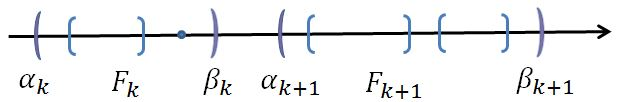
\includegraphics[width=0.5\textwidth]{image/ClosedSet2.jpg}
\end{figure}

\vspace*{-0.3cm}

注意到
\[
F = F \cap \big(\medcup\limits_{k=1}^n (\alpha_k,\,\beta_k)\big) =
\medcup\limits_{k=1}^n \big(F \cap (\alpha_k,\,\beta_k)\big) = \medcup\limits_{k=1}^n F_k
\]
由于~$\{F_k\}$~为互不相交的闭集, 由命题~\ref{prop223}
\begin{eqnarray} \label{eq221}
m(F) &=& m \Big(\medcup_{k=1}^n F_k \Big) = \sum_{k=1}^n m(F_k) \nonumber \\
&=& \sum_{k=1}^n (\beta_k - \alpha_k) - \sum_{k=1}^n m\big((\alpha_k,\,\beta_k)
- F_k\big) \\
&=& m(G) - \sum_{k=n+1}^\infty (\beta_k - \alpha_k) -
\sum_{k=1}^n m\big((\alpha_k,\,\beta_k) - F_k\big) \nonumber
\end{eqnarray}
并且
\[
G-F = \medcup\limits_{k=1}^n \big((\alpha_k,\,\beta_k) - F_k\big)
\medcup \big({\medcup\limits_{k=n+1}^\infty} (\alpha_k,\,\beta_k)\big)
\]
由于它们是互不相交的开集, 故由命题~\ref{prop221}
\begin{eqnarray} \label{eq222}
m(G-F) &=& m\big( \medcup_{k=1}^n \big((\alpha_k,\,\beta_k) - F_k\big) \big) +
m\big( \medcup_{k=n+1}^\infty (\alpha_k,\,\beta_k) \big) \nonumber \\
&=& \sum_{k=n+1}^\infty (\beta_k - \alpha_k) + \sum_{k=1}^n m\big((\alpha_k,\,\beta_k)
- F_k\big)
\end{eqnarray}
由式~\eqref{eq221},\,\eqref{eq222}~得, $m(G-F) = m(G) - m(F)$.
\end{proof}

\section{一维有界集的外测度、内测度}

\subsection{一维有界集的外测度}

\begin{definition}
设~$E \subset \R$~为有界集, 则~$E$~的外测度\index{外测度}定义为包含~$E$~的开集测度的下确界,
记为~$m^*(E)$, 即
\[
m^*(E) = \inf\big\{m(G): \: G \supset E,\, G \mbox{~开}\big\}
\]
\end{definition}

\begin{remark} \label{rem231}
(i) $E \subset \R$~有界, 则存在开区间~$(a,\,b) \supset E$,
即
\[
(a,\,b) \in \{G: \: G \supset E,\, G \mbox{~开}\}
\]
故~$m^*(E) \leqslant b - a < +\infty$. 从而上述定义有意义.

(ii) 任意一维有界集都有外测度, 若~$E$~是开集, 由开集测度的单调性
可得~$m^*(E) = m(E)$.
\end{remark}

\begin{theorem} \label{thm231}
设~$E \subset \R$~为有界集, 则存在单调递减开集列~$G_n$~满足~$G_n \supset E$,
且~$\lim\limits_{n \to \infty} m(G_n) = m^*(E)$.
\end{theorem}

\begin{proof}
$m^*(E) = \inf\{m(G): \: G \supset E,\, G \mbox{~开}\}$, 由~``$\inf$''~的定义,
对~$\varepsilon_1 = 1$, 存在开集~$G_1 \supset E$~使得
\[
m^*(E) \leqslant m(G_1) < m^*(E) + 1
\]
对~$\varepsilon_2 = 1/2$, 存在开集~$G'_2 \supset E$~使得
\[
m^*(E) \leqslant m(G'_2) < m^*(E) + \frac{1}{2}
\]
令~$G_2 = G'_2 \cap G_1$, 则~$G_2$~是开集, $G_2 \supset E$, 且
\[
m^*(E) \leqslant m(G_2) < m^*(E) + \frac{1}{2}
\]
依次做下去, 得到单调递减的开集列~$\{G_n\}$~满足~$G_n \supset E$, 且
\[
m^*(E) \leqslant m(G_n) < m^*(E) + \frac{1}{n}, \quad n = 1,\,2,\,\cdots
\]
两边取极限得~$m^*(E) = \lim\limits_{n \to \infty} m(G_n)$.
\end{proof}

\subsection{一维有界集外测度的性质}

\begin{proposition}[外测度性质]
设~$E,\,E_1,\,E_2,\,E_k$~为~$\R$~中的有界集, 则它们具有如下性质:

(i) (\textbf{非负性}) $m^*(E) \geqslant 0$;

(ii) (\textbf{单调性}) 若~$E_1 \subset E_2$, 则~$m^*(E_1) \leqslant m^*(E_2)$;

(iii) (\textbf{次可加性}) $m^*\big( \smallcup\limits_{k=1}^\infty E_k \big) \leqslant \sum\limits_{k=1}^\infty m^*(E_k)$.
\end{proposition}

\begin{proof}
(i), (ii)~显然.

(iii) 不妨设~$m^*(E_k) < +\infty, \, \forall~k \in \N$. 由外测度定义,
对~$\forall~\varepsilon > 0$, 存在开集~$G_k \supset E_k$~使得
\[
m(G_k) < m^*(E_k) + \frac{\varepsilon}{2^k}, \quad \forall~k \in \N
\]
令~$G = \smallcup\limits_{k=1}^\infty G_k$, 则~$G$~是开集, 且~$G \supset
\smallcup\limits_{i=1}^\infty E_k$. 故
\[
m^*\Big(\medcup^\infty_{k=1} E_k\Big) \leqslant m(G) \leqslant \sum^\infty_{k=1}m(G_k)
< \sum^\infty_{k=1} m^*(E_k) + \varepsilon
\]
由~$\varepsilon$~的任意性可得~$m^*\Big( \smallcup\limits_{k=1}^\infty E_k \Big) \leqslant
\sum\limits_{k=1}^\infty m^*(E_k)$.
\end{proof}

\medskip

\begin{example} \label{ex231}
若~$E$~是可数集, 则~$m^*(E) = 0$.
\end{example}

\medskip

\begin{proof}
不妨设~$E = \{x_n\}^\infty_{n=1}$, 对~$\forall~\varepsilon > 0$, 令
~$E_\varepsilon = \smallcup\limits_{n=1}^\infty \big(x_n-\varepsilon/2^{n+1},\,x_n+\varepsilon/2^{n+1}\big)$.
则~$E_\varepsilon$~是开集, 且~$E_\varepsilon \supset E$. 故
\[
m^*(E) \leqslant m(E_\varepsilon) = \sum_{n=1}^\infty \Big(2 \cdot
\frac{\varepsilon}{2^{n+1}} \Big) = \varepsilon
\]
由~$\varepsilon$~的任意性以及外测度的非负性得, $m^*(E) = 0$.
\end{proof}

\begin{theorem}
设~$E_1,\,E_2$~为~$\R$~中的有界集, 若~$d(E_1,\,E_2) > 0$, 则\footnote{外测度满足该定理条件, 也称其满足距离外测度性质. }
\[
m^*(E_1 \cup E_2) = m^*(E_1) + m^*(E_2)
\]
\end{theorem}

\begin{proof}
只需证明~$m^*(E_1) + m^*(E_2) \leqslant m^*(E_1 \cup E_2)$. 由外测度的定义,
对任意开集~$G \supset E$, $m^*(E)$~可表示为
\[
m^*(E) = \inf\{m(E'): \: E \subset E' \subset G, \, E' \mbox{~开}\}
\]
由于~$d(E_1,\,E_2)>0$, 由定理~\ref{thm1.4.10}, 则存在开集~$G_1,\,G_2$~
使得~$E_1 \subset G_1,\,
E_2\subset G_2$, 且~$G_1 \cap G_2 = \emptyset$. 从而
\begin{eqnarray*}
&& m^*(E_1)+m^*(E_2) \\
&=& \inf\big\{m(E'_1):\:E_1 \subset E'_1 \subset G_1,\, E'_1 \mbox{~开}\big\} + \inf\big\{m(E'_2):\:E_2 \subset E'_2 \subset G_2,\, E'_2 \mbox{~开}\big\} \\
&\leqslant& \inf\big\{m(E'_1)+m(E'_2):\:E_i \subset E'_i \subset G_i,\, E'_i \mbox{~开},
\,i=1,\,2\big\} \\
&=& \inf\big\{m(E'_1 \cup E'_2): \: (E_1 \cup E_2) \subset (E'_1 \cup E'_2) \subset
(G_1 \cup G_2),\,(E'_1 \cup E'_2) \mbox{~开}\big\} \\
&=& m^*(E_1 \cup E_2)
\end{eqnarray*}
定理得证.
\end{proof}

注意: 若定理条件减弱为~``$E_1 \cap E_2 = \emptyset$'', 则结论不一定成立.

\begin{theorem}[外测度平移不变性\index{外测度平移不变性}]
设~$E$~为~$\R$~中的有界集, $x_0 \in \R$, 则
\[
m^*\big(E + \{x_0\} \big) = m^*(E)
\]
\end{theorem}

\begin{proof}
若~$G$~是包含~$E$~的开集, 则~$G + \{x_0\}$~是包含~$E + \{x_0\}$~的开集,
且从~$G$~到~$G + \{x_0\}$~只是构成区间平移了~$x_0$~个单位, 区间长度并未发生变化.
由外测度的定义知定理结论成立.
\end{proof}

\subsection{一维有界集的内测度及性质}

\begin{definition}
设~$E \subset \R$~为有界集, 则~$E$~的内测度\index{内测度}定义为含于~$E$~的闭集测度的上确界,
记为~$m_*(E)$, 即
\[
m_*(E) = \sup \big\{m(F): \: F \subset E,\, F \mbox{~闭}\big\}
\]
\end{definition}

\begin{remark} \label{rem233}
任意一维有界集都有内测度, 若~$E$~是闭集, 由闭集测度单调性可得~$m_*(E) = m(E)$.
\end{remark}

\begin{proposition}
由内测度的定义, 易知~$\R$~上的内测度具有如下性质:

(i) (\textbf{非负性}) $m_*(E) \geqslant 0$;

(ii) (\textbf{单调性}) 若~$E_1 \subset E_2$, 则~$m_*(E_1) \leqslant m_*(E_2)$.
\end{proposition}

\begin{theorem}
设~$E \subset \R$~为有界集, 则存在单调递增闭集列~$F_n$~满足~$F_n \subset E$,
且~$\lim\limits_{n \to \infty} m(F_n) = m_*(E)$.
\end{theorem}

\begin{proof}
类似定理~\ref{thm221}~可证.
\end{proof}

\begin{proposition}
设~$E \subset \R$~为有界集, 则~$m_*(E) \leqslant m^*(E)$.
\end{proposition}

\begin{proof}
对任意有界开集~$G \supset E$, 闭集~$F \subset E$~都有~$F \subset E \subset G$,
故~$F \subset G$. 由引理~\ref{lem223}, $m(F) \leqslant m(G)$. 固定~$F$, 对~$G$~取~``$\inf$''~得
~$m(F) \leqslant m^*(E)$. 再对~$F$~取~``$\sup$''~得~$m_*(E) \leqslant m^*(E)$.
\end{proof}



\section{一维有界可测集及性质}

\subsection{一维有界可测集}

\begin{definition}
设~$E \subset \R$~为有界集, 若~$m_*(E) = m^*(E)$, 则称~$E$~为勒贝格可测集, 简称可测集\index{可测集}, 其测度记为~$m(E)$.
\end{definition}
\begin{remark}
一维有界开集、闭集都是可测集, 其测度就是~\S~2.1~中定义的测度.
\end{remark}

\begin{proof}
若~$G \subset \R$~为有界开集, 则由注~\ref{rem231}~和定理~\ref{thm221}~得~$m^*(G) = m(G) = m_*(G)$. 若~$F \subset \R$~为有界闭集,
则由注~\ref{rem233}~和定理~\ref{thm222}~得~$m_*(F) = m(F) = m^*(F)$.
\end{proof}

\begin{definition}
测度为~$0$~的集合, 称为零测集\index{零测集}.
\end{definition}

\begin{theorem}
零测集的任意子集可测, 且也是零测集.
\end{theorem}

\begin{proof}
设~$m(E) = 0, \, E_0 \subset E$, 则
\[
0 \leqslant m_*(E_0) \leqslant m^*(E_0) \leqslant m^*(E) = m(E) = 0
\]
故~$m(E_0) = m_*(E_0) = m^*(E_0) = 0$.
\end{proof}

\medskip

\begin{example}
设~$E$~是可数集, 则~$m(E) = 0$.
\end{example}

\medskip

\begin{proof}
由~\S~2.2~例~\ref{ex231}~知, $m^*(E) = 0$. 又~$0 \leqslant m_*(E) \leqslant m^*(E) =0$,
故~$m(E) = m_*(E) = m^*(E) =0$.
\end{proof}

\begin{theorem} \label{thm0}
可数个零测集的并是零测集.
\end{theorem}

\begin{proof}
设~$E_1,\,E_2,\,\cdots,\, E_n, \, \cdots$~是零测集, 记~$E = \smallcup\limits_{n=1}^\infty
E_n$. 由外测度定义, 对~$\forall~\varepsilon > 0$, 以及~$n \in \N$, 都存在开集~
$G_n \supset E_n$~满足
\[
m(G_n) < m^*(E_n) + \frac{\varepsilon}{2^n} = m(E_n) + \frac{\varepsilon}{2^n}
= \frac{\varepsilon}{2^n}
\]
令~$G = \smallcup\limits_{n=1}^\infty G_n$, 则~$G$~开, $G \supset E$, 且
\[
m^*(E) \leqslant m(G) \leqslant \sum_{n=1}^\infty m(G_n) < \varepsilon
\]
由~$\varepsilon$~的任意性, $m^*(E) = 0$, 从而~$m(E) = 0$.
\end{proof}

\begin{theorem} \label{thm242}
设~$E \subset \R$~为有界集, $E_0$~为零测集, 则:

(i) $m^*(E \cup E_0) = m^*(E)$;

(ii) $m_*(E \cup E_0) = m_*(E)$.
\end{theorem}

\begin{proof}
(i) 对~$\forall~\varepsilon > 0$, 取开集~$G \supset E,\,G_0 \supset E_0$~满足
\[
m(G) \leqslant m^*(E) + \frac{\varepsilon}{2}, \quad m(G_0) < \frac{\varepsilon}{2}
\]
则开集~$G \cup G_0 \supset E \cap E_0$, 且
\[
m(G \cup G_0) \leqslant m(G) + m(G_0) < m^*(E) + \varepsilon
\]
由~$\varepsilon$~的任意性, $m(G \cup G_0) \leqslant m^*(E)$, 再由外测度的定义
\[
m^*(E \cup E_0) \leqslant m(G \cup G_0) \leqslant m^*(E)
\]
而相反的不等式显然, 因此, $m^*(E \cup E_0) = m^*(E)$.

(ii) 设~$\varepsilon,\,G_0$~如~(i)~所述, 任取闭集~$F \subset E \cup E_0$, 则
\begin{eqnarray*}
m_*(F) &=& m_*\big((F - G_0) \cup G_0 \big) \leqslant m^*\big((F - G_0) \cup G_0 \big) \\
&\leqslant& m^*(F - G_0) + m^*(G_0)
\end{eqnarray*}
注意到~$F$~闭, $F - G_0$~闭, 且~$F - G_0 \subset E$,\, $G_0$~开, 故它们都是可测集, 于是
\[
m(F) \leqslant m(F-G_0) + m(G_0) < m_*(E) + \frac{\varepsilon}{2}
\]
由~$\varepsilon$~的任意性, $m(F) \leqslant m^*(E)$, 对闭集~$F$~取~``$\sup$''~得
\[
m_*(E \cup E_0) \leqslant m_*(E)
\]
而相反的不等式显然, 因此, $m_*(E \cup E_0) = m_*(E)$.
\end{proof}

由定理~\ref{thm242}, 对于~$\R$~中任意有界集~$E$, 并上零测集~$E_0$~不改变~$E$~的外测度和内测度, 从而:

\begin{corollary}
$\R$~中有界集并上零测集不改变可测性, 即若~$E$~不可测, 则~$E \cup E_0$~也不可测;
若~$E$~可测, 则~$E \cup E_0$~也可测, 且~$m(E \cup E_0) = m(E)$.
\end{corollary}

\begin{theorem} \label{thm243}
设~$E$~为~$\R$~中的有界集, 则~$E$~可测, 当且仅当存在开集~$G \supset E$,
闭集~$F \subset E$, 使得~$m(G-F) < \varepsilon$.
\end{theorem}

\begin{proof}
``$\Rightarrow$''. $E$~可测, 则~$m^*(E) = m_*(E) = m(E)$, 故对~$\forall~\varepsilon > 0$,
存在开集~$G \supset E$, 闭集~$F \subset E$~使得
\[
m(G) < m^*(E) + \frac{\varepsilon}{2} = m(E) + \frac{\varepsilon}{2}
\]
\[
m(F) > m_*(E) - \frac{\varepsilon}{2} = m(E) - \frac{\varepsilon}{2}
\]
从而由定理~\ref{thm223}, $m(G-F) = m(G)-m(F) < \varepsilon$.

``$\Leftarrow$''. 设对~$\forall~\varepsilon > 0$, 存在开集~$G \supset E$,
闭集~$F \subset E$~
使得~$m(G-F) < \varepsilon$. 由定理~\ref{thm223}, $m(G) - m(F) < \varepsilon$. 又
\[
m(F) \leqslant m_*(E) \leqslant m^*(E) \leqslant m(G)
\]
故~$m^*(E) - m_*(E) < \varepsilon$. 由~$\varepsilon$~的任意性,
则有~$m^*(E) \leqslant m_*(E)$. 而~$m^*(E) \geqslant m_*(E)$~总成立, 故~$m^*(E) = m_*(E)$,
从而~$E$~可测.
\end{proof}

\subsection{一维有界可测集的性质}

设下文中出现的集~$E,\,E_1,\,E_2,\,E_k$~等都是一维有界集.

\begin{proposition}[非负性]
$m(E) \geqslant 0$.
\end{proposition}

\begin{proposition}[平移不变性]
$m\big(E + \{x_0\} \big) = m(E)$.
\end{proposition}

\begin{proof}
由于~$m(E) = m^*(E)$, 再由外测度平移不变性可得.
\end{proof}

\begin{proposition}[集运算封闭性Ⅰ] \label{prop242}

(i) 设~$X = (a,\,b)$~为全集, 若~$E$~可测, 则~$E^c$~可测;

(ii) 若~$E_1,\,E_2$~可测, 则~$E_1 \cup E_2,\,E_1 \cap E_2,\,
E_1 - E_2$~都可测; 若~$E_1 \cap E_2 = \emptyset$, 则~$m(E_1 \cup E_2) = m(E_1) + m(E_2)$.
\end{proposition}

\begin{proof}
(i) $E$~可测, 由可测集等价定义, 对~$\forall~\varepsilon > 0$,
存在开集~$G \supset E$~与闭集~$F \subset E$, 使得~$m(G-F) < \varepsilon$.

则~$G^c$~闭满足~$G^c \subset E^c$, $F^c$~开满足~$F^c \supset E^c$, 并且
\[
F^c - G^c = \big[(a,\,b)-F\big] - \big[(a,\,b)-G\big] = G - F
\]
故~$m(F^c - G^c) = m(G - F) < \varepsilon$. 由可测集等价定义, $E^c$~可测.

(ii) $E_1,\,E_2$~可测, 由定理~\ref{thm243}, 存在开集~$G_i$, 闭集~$F_i$, 使得
\[
G_i \supset E_i \supset F_i, \quad m(G_i - F_i) < \varepsilon, \quad i = 1,\,2
\]
令~$G = G_1 \cup G_2,\,F = F_1 \cup F_2$, 则~$G \supset (E_1 \cup E_2) \supset F$, 且
\[
G-F \subset (G_1 - F_1) \cup (G_2 - F_2)
\]
从而
\begin{eqnarray*}
m(G-F) &\leqslant& m\big( (G_1 - F_1) \cup (G_2 - F_2) \big) \\
&\leqslant& m(G_1 - F_1) + m(G_2 - F_2) \\
&<& 2 \varepsilon
\end{eqnarray*}
由定理~\ref{thm243}, $E_1 \cup E_2$~可测.

若~$E_1 \cap E_2 = \emptyset$, 则~$F_1 \cap F_2 = \emptyset$. 由命题~\ref{prop223}
\begin{eqnarray*}
m(E_1 \cup E_2) &\geqslant& m(F_1 \cup F_2) = m(F_1) + m(F_2) \\
&>& m(G_1) + m(G_2) - 2 \varepsilon \\
&\geqslant& m(E_1) + m(E_2) - 2 \varepsilon
\end{eqnarray*}
由~$\varepsilon$~的任意性, $m(E_1 \cup E_2) \geqslant m(E_1) + m(E_2)$. 另一方面
\begin{eqnarray*}
m(E_1 \cup E_2) &\leqslant& m(G_1 \cup G_2) \leqslant m(G_1) + m(G_2) \\
&<& m(F_1) + m(F_2) + 2 \varepsilon \\
&\leqslant& m(E_1) + m(E_2) + 2 \varepsilon
\end{eqnarray*}
由~$\varepsilon$~的任意性得
\[
m(E_1 \cup E_2) \leqslant m(E_1) + m(E_2)
\]
综上~$m(E_1 \cup E_2) = m(E_1) + m(E_2)$.

注意到~$E_1 \cap E_2 = \big(E_1^c \cup E_2^c\big)^c$, 故~$E_1 \cap E_2$~可测.
再由~$E_1 - E_2 = E_1 \cap E_2^c$~知, $E_1 - E_2$~可测.
\end{proof}

\begin{remark} \label{rem242}
设~$X = (a,\,b)$~为全集, $E \subset X$, 则~$m(E^c) = b-a - m(E)$.
\end{remark}

\begin{proof}
由命题~\ref{prop242}~(ii), $m\big( (a,\,b) \big) = m(E \cup E^c) = m(E) + m(E^c)$.
注意到~$m(E) < +\infty$, 故
\[
m(E^c) = m\big( (a,\,b) \big) - m(E) = b-a - m(E)
\]
\end{proof}

\begin{proposition}[单调性]
设~$E_1,\,E_2$~可测, 且~$E_1 \subset E_2$, 则~$m(E_1) \leqslant m(E_2)$.
\end{proposition}

\begin{proof}
由命题~\ref{prop242}~(ii), $E_2 - E_1$~可测. 又~$E_2 = E_1 \cup (E_2 - E_1)$~且
~$E_1 \cap (E_2 - E_1) = \emptyset$, 注意到测度的非负性, 再由命题~\ref{prop242}~(ii)~得
\[
m(E_2) = m(E_1) + m(E_2 - E_1) \geqslant m(E_1)
\]
\end{proof}

\begin{proposition}[集运算封闭性Ⅱ] \label{prop244}

(i) 设~$E_1,\,E_2,\,\cdots$~可测, 则~$\smallcup\limits_{k=1}^\infty
E_k$~可测, 且满足次可加性
\[
m\big( \medcup_{k=1}^\infty E_k \big) \leqslant \sum_{k=1}^\infty m(E_k)
\]
若~$E_k$~互不相交, 则
\[
m\big( \medcup_{k=1}^\infty E_k \big) = \sum_{k=1}^\infty m(E_k)
\]

(ii) 设~$E_1,\,E_2,\,\cdots$~可测, 则~$\smallcap\limits_{k=1}^{\infty}E_k$~可测.
\end{proposition}

\begin{proof}
(i) 设~$E_1,\,E_2,\,\cdots$~可测, 记~$E = \smallcup\limits_{k=1}^\infty E_k$.

若~$E_k$~互不相交, 由命题~\ref{prop242}~易知, 对~$\forall~n \in \N$,
都有~$\smallcup\limits_{k=1}^n E_k$~可测, 且~$m\big( \smallcup\limits_{k=1}^n E_k \big)
= \sum\limits_{k=1}^n m(E_k)$. 故对~$\forall~\varepsilon > 0$, 存在闭集
~$F \subset \smallcup\limits_{k=1}^n E_k$, 使得
\[
m(F) > m_*\big( \medcup\limits_{k=1}^n E_k \big) - \varepsilon = m\big( \medcup\limits_{k=1}^n E_k \big) - \varepsilon
\]
故
\[
m_*(E) \geqslant m(F) > m\big( \medcup_{k=1}^n E_k \big) - \varepsilon =
\sum_{k=1}^n m(E_k) - \varepsilon
\]
由~$\varepsilon$~的任意性, $m_*(E) \geqslant \sum\limits_{k=1}^n m(E_k)$. 令~$n \to \infty$~得
~$m_*(E) \geqslant \sum\limits_{k=1}^\infty m(E_k)$.

另一方面, 对~$\forall~\varepsilon > 0$~及每个~$k$, 作开集~$G_k \supset E_k$, 满足
\[
m(G_k) < m^*(E_k) + \frac{\varepsilon}{2^k} = m(E_k) + \frac{\varepsilon}{2^k}
\]
令~$G = \smallcup\limits_{k=1}^\infty G_k$, 则~$G$~开, 且~$G \supset E$. 故
\[
m^*(E) \leqslant m(G) \leqslant \sum_{k=1}^\infty m(G_k) < \sum_{k=1}^\infty m(E_k)
+ \varepsilon
\]
由~$\varepsilon$~的任意性, $m^*(E) \leqslant \sum\limits_{k=1}^\infty m(E_k)$.
综上再由~$m_*(E) \leqslant m^*(E)$~可得, $m(E) = \sum\limits_{k=1}^\infty m(E_k)$.

若~$E_k$~相交, 则
\[
E = E_1 \cup (E_2 - E_1) \cup (E_3 - E_2 - E_1) \cup \cdots
\]
可测.

(ii) $\smallcap\limits_{k=1}^\infty E_k = \big( \smallcup\limits_{k=1}^\infty
E_k^c \big)^c$~可测.
\end{proof}

\begin{proposition}[单调集列测度的极限性质\index{单调集列测度的极限性质}] \label{prop245}

(i) 设~$\{E_k\}$~为单调递增的可测集列, 则~$E =\smallcup\limits_{k=1}^\infty E_k$~可测, 且
\[
m\big( \lim_{k \to \infty} E_k \big) = m(E) = \lim_{k \to \infty} m(E_k)
\]

(ii) 设~$\{E_k\}$~为单调递减的可测集列, 则~$E = \smallcap\limits_{k=1}^\infty E_k$~可测, 且
\[
m\big( \lim_{k \to \infty} E_k \big) = m(E) = \lim_{k \to \infty} m(E_k)
\]
\end{proposition}

\begin{proof}
(i) 由命题~\ref{prop244}, $E$~可测. 又~$E$~可分解为如下互不相交集的并
\[
E = E_1 \cup (E_2 - E_1) \cup \cdots \cup (E_k - E_{k-1}) \cup \cdots
\]
由于
\[
m(E_k) = m\big((E_k - E_{k-1}) \cup E_{k-1}\big) = m(E_k - E_{k-1}) + m(E_{k-1})
\]
注意到~$m(E_{k-1}) < +\infty$, 故~$m(E_k - E_{k-1}) = m(E_k) - m(E_{k-1})$.
于是由命题~\ref{prop244}~得
\begin{eqnarray*}
m(E) &=& m(E_1) + \sum_{k=2}^\infty m(E_k - E_{k-1}) \\
&=& m(E_1) + \sum_{k=2}^\infty \big(m(E_k) - m(E_{k-1})\big) \\
&=& \lim_{k \to \infty} m(E_k)
\end{eqnarray*}

(ii) 设~$X = (a,\,b)$~为全集. $\{E_k\}$~单调递减, 则~$\{E_k^c\}$~单调递增.
又~$E^c = \smallcup\limits_{k=1}^\infty E_k^c$, 应用~(i)~得~$m(E^c) =
\lim\limits_{k \to \infty} m(E_k^c)$. 由注~\ref{rem242}~得
\[
b-a - m(E) = \lim\limits_{k \to \infty} \big( b-a - m(E_k) \big)
\]
因此, $m(E) = \lim\limits_{k \to \infty} m(E_k)$.
\end{proof}

\subsection{测度的另一种定义}

\begin{lemma} \label{lem241}
设~$E \subset (a,\,b)$, 则~$m_*(E) + m^*(E^c) = b-a$.
\end{lemma}

\begin{proof}
对~$\forall~\varepsilon > 0$, 取闭集~$F \subset E$~满足~$m(F) > m_*(E) - \varepsilon$.
又~$F^c$~开, 且~$F^c \supset E^c$, 故由注~\ref{rem242}~得
\[
m^*(E^c) \leqslant m(F^c) = b-a - m(F)
\]
从而~$m_*(E) + m^*(E^c) < b-a + \varepsilon$. 由~$\varepsilon$~的任意性,
$m_*(E) + m^*(E^c) \leqslant b-a$.

另一方面, 设~$X = (a,\,b)$~为全集, 不妨设既开又闭. 

对~$\forall~\varepsilon > 0$, 取开集~$G \supset E^c$~满足~$m(G) < m^*(E^c) + \varepsilon$. 
又~$G^c$~闭, 且~$G^c \subset E$, 故
\[
m_*(E) \geqslant m(G^c) = b-a - m(G)
\]
从而~$m_*(E) + m^*(E^c) > b-a - \varepsilon$. 由~$\varepsilon$~的任意性,
$m_*(E) + m^*(E^c) \geqslant b-a$.

综上可得~$m_*(E) + m^*(E^c) = b-a$.
\end{proof}

\begin{theorem} \label{thm244}
设~$E \subset \R$~为有界集, 则~$E$~可测~$\Leftrightarrow$~对任意点集~
$T \subset \R$, 都有
\begin{equation} \label{eq21}
m^*(T) = m^*(T \cap E) + m^*(T \cap E^c)
\end{equation}
\end{theorem}

\begin{proof}
``$\Rightarrow$''.\ 设~$T$~为~$\R$~中的有界点集,
对~$\forall~\varepsilon > 0$, 由外测度定义, 存在开集~$G \supset T$~
使得~$m(G) < m^*(T) + \varepsilon$. 由于~$G \cap E \supset T \cap E,\,
G \cap E^c \supset T \cap E^c$, 故
\[
m^*(T \cap E) \leqslant m^*(G \cap E) = m(G \cap E)
\]
\[
m^*(T \cap E^c) \leqslant m^*(G \cap E^c) = m(G \cap E^c)
\]
注意到~$G \cap E$~与~$G \cap E^c$~互不相交, 则有
\[
m(G \cap E) + m(G \cap E^c) = m\big( (G \cap E) \cup (G \cap E^c) \big) = m(G)
\]
从而
\begin{eqnarray*}
m^*(T) &>& m(G) - \varepsilon \\
&=& m(G \cap E) + m(G \cap E^c) - \varepsilon \\
&\geqslant& m^*(T \cap E) + m^*(T \cap E^c) - \varepsilon
\end{eqnarray*}
由~$\varepsilon$~的任意性, $m^*(T) \geqslant m^*(T \cap E) + m^*(T \cap E^c)$.

另一方面, 由外测度的次可加性
\begin{eqnarray*}
m^*(T) &=& m^*\big( T \cap (E \cup E^c) \big) \\
&=& m^*\big( (T \cap E) \cup (T \cap E^c) \big) \\
&\leqslant& m^*(T \cap E) + m^*(T \cap E^c)
\end{eqnarray*}

综上可得~$m^*(T) = m^*(T \cap E) + m^*(T \cap E^c)$.

\smallskip

``$\Leftarrow$''.\ 设~$X = (a,\,b)$~为全集, 取~$T = (a,\,b)$, 则由条件~\eqref{eq21}
\[
b - a = m^*\big( (a,\,b) \big) = m^*(E) + m^*(E^c)
\]
故由引理~\ref{lem241}, $m^*(E) = b - a - m^*(E^c) = m_*(E)$. 因此, $E$~可测.
\end{proof}

\begin{remark}
(i) 条件~\eqref{eq21}~又称为卡拉西尔德瑞条件\index{卡拉西尔德瑞条件}, 许多实变函数教材把
定理~\ref{thm244}~作为勒贝格可测集的原始定义;

(ii) 由引理~\ref{lem241}, 有界集~$E$~的内测度可以表示为:
$m_*(E) = b - a - m^*(E^c)$. 可见, 一维有界集~$E$~的内测度、测度
都可以用外测度来定义.
\end{remark}

\subsection{波雷尔集}

下面讨论~$\R$~中可测集\footnote{~这里不区分有界、无界, 一维无界集的测度定义见~\S2.4.}的构造问题, 即~$\R$~中哪些点集是可测的？能否对可测集给出一种相对直观的描述？

我们知道, 一维开集、闭集是可测集, 由命题~\ref{prop244}, 可列个开集的并(是开集)、可列个开集的交、可列个闭集的并、可列个闭集的交(是闭集)仍是可测集.

\begin{definition}
可列个开集的交, 称为~$G_\delta$~集\index{$G_\delta$~集}; 可列个闭集的并,
称为~$F_\sigma$~集\index{$F_\sigma$~集}.
可见~$G_\delta$~集的余集是~$F_\sigma$~集; $F_\sigma$~集的余集是~$G_\delta$~集.
\end{definition}

\medskip

\begin{example}
有理数点集~$\Q$~可表示为~$\smallcup\limits_{k=1}^\infty \{r_k\}$,
从而是~$F_\sigma$~集.
\end{example}

\medskip

\begin{example}
设~$f(x)$~为定义在开集~$G \subset \R$~上的实值函数, 则~$f(x)$~的连续点集
是~$G_\delta$~集.
\end{example}

\medskip

\begin{proof}
记~$\omega(x)$~为~$f$~在点~$x$~的振幅, 则~$f(x)$~在~$x = x_0$~处连续的充要条件\footnote{该结论的证明见第四章第~4~节. }是
~$\omega(x_0) = 0$. 故~$f(x)$~的连续点集可表示为
\[
\medcap_{k=1}^\infty \Big\{ x \in G: \: \omega(x) < \frac{1}{k} \Big\}
\]
由于~$\{ x \in G: \: \omega(x) < 1/k \}$~是开集, 故~$f(x)$~的连续点集是~$G_\delta$~集.
\end{proof}

\begin{definition}
由~$\R$~中的开集、闭集, 经过至多可列次``并、交、差''~的运算得到的集合,
称为波雷尔集\index{波雷尔集}.
\end{definition}

波雷尔集, 也可以用~$\sigma$-代数\index{$\sigma$-代数}的方式定义如下:


\begin{definition}
设~$\mathnormal{\Gamma}$~是由~$X$~的子集构成的集族, 且满足:

(i) $\emptyset \in {\mathnormal\Gamma}$;

(ii) 若~$A \in {\mathnormal\Gamma}$, 则~$A^c \in {\mathnormal\Gamma}$;

(iii) 若~$A_n \in {\mathnormal\Gamma}, \, n = 1,\,2,\,\cdots$, 则~$\smallcup
\limits_{n = 1}^\infty A_n \in {\mathnormal\Gamma}$.
则称~${\mathnormal\Gamma}$~是一个~$\sigma$-代数.
\end{definition}

由~$\sigma$-代数的定义易知:
\begin{publist}
\item[(1)] 若~$A_n \in {\mathnormal\Gamma}, \, n = 1,\,\cdots, \, m$, 则~$\smallcup
\limits_{n = 1}^m A_n \in {\mathnormal\Gamma}$;
\item[(2)] 若~$A_n \in {\mathnormal\Gamma}, \, n = 1,\,2,\,\cdots$, 则
\[
\medcap_{n = 1}^\infty A_n \in {\mathnormal\Gamma}, \quad \limsup_{n \to \infty} A_n \in {\mathnormal\Gamma},
\quad \liminf_{n \to \infty} A_n \in {\mathnormal\Gamma}
\]
\item[(3)] 若~$A,\,B \in {\mathnormal\Gamma}$, 则~$A - B \in {\mathnormal\Gamma}$;
\item[(4)] $X \in {\mathnormal\Gamma}$.
\end{publist}

设~${\mathnormal\Sigma}$~是由~$X$~的子集构成的集族, 包含~${\mathnormal\Sigma}$~的最小
\footnote{按集合包含关系: ${\mathnormal\Sigma}_1 \preccurlyeq {\mathnormal\Sigma}_2 \Leftrightarrow {\mathnormal\Sigma}_1
\subset {\mathnormal\Sigma}_2$. }~$\sigma$-代数, 称为由~${\mathnormal\Sigma}$~生成的~$\sigma$-代数.

由~$\R$~中所有开集构成的开集族所生成的~$\sigma$-代数, 称为波雷尔
集类, 记为~$\mathfrak{B}(\R)$. $\mathfrak{B}(\R)$~中的元素,
称为波雷尔集.

显然, 开集、闭集、$G_\delta$~集、$F_\sigma$~集都是波雷尔集; 波雷尔集的余集是波雷尔集;
波雷尔集的有限或可列交、并是波雷尔集; 波雷尔集的上、下限集是波雷尔集.

\begin{theorem}
任意波雷尔集都是可测集.
\end{theorem}

\begin{theorem} \label{thm246}
设~$E \subset \R$~可测, 则存在~$G_\delta$~集~$A$~以及~$F_\sigma$~集~$B$,
使得~$A \supset E \supset B$~且~$m(A) = m(E) = m(B)$.
\end{theorem}

\begin{proof}
设~$E$~可测, 由外测度定义, 对每个~$n \in \N$, 存在开集~$G_n \supset E$~使得
\[
m(G_n) < m^*(E) + \frac{1}{n} = m(E) + \frac{1}{n}
\]
令~$A = \smallcap\limits_{n=1}^\infty G_n$, 则~$A$~是~$G_\delta$~集. 由于~$E \subset
A \subset G_n$, 故由测度的单调性
\[
0 \leqslant m(A) - m(E) \leqslant m(G_n) - m(E) < \frac{1}{n}
\]
令~$n \to \infty$~得, $m(A) = m(E)$.

由内测度的定义, 对每个~$n \in \N$, 存在闭集~$F_n \subset E$~使得
\[
m(F_n) > m_*(E) - \frac{1}{n} = m(E) - \frac{1}{n}
\]
令~$B = \smallcup\limits_{n=1}^\infty F_n$, 则~$B$~是~$F_\sigma$~集. 由于~$F_n \subset
B \subset E$, 故由测度的单调性
\[
0 \leqslant m(E) - m(B) \leqslant m(E) - m(F_n) < \frac{1}{n}
\]
令~$n \to \infty$~得, $m(B) = m(E)$.
\end{proof}

\begin{remark}
从前面定理证明可看出, 若~$E$~可测, 则存在~$G_\delta$~集~$A$~以及~$F_\sigma$~集~$B$,
使得~$A \supset E \supset B$~且~$m(A) = m^*(E),\, m(B) = m_*(E)$.
\end{remark}

由定理~\ref{thm246}, $\R$~中的可测集~$E$~与某个~$G_\delta$~集以及
某个~$F_\sigma$~集只相差一个零测集. 反过来, 某个$G_\delta$~集或~$F_\sigma$~集
并上零测集仍是可测集. 因此, 我们得到~$\R$~中可测集的一种构造:

\begin{theorem}
可测集~$=$~波雷尔集~$\smallcup$~零测集.
\end{theorem}

那么是否存在不是波雷尔集的可测集呢? 回答是肯定的, 下面给出这样一个例子.

\begin{lemma} \label{lem232}
设~$f(x)$~为定义在~$E \subset \R^n$~上的实值函数, ${\mathnormal\Gamma}$~为~$\R^n$~中一些子集构成的~$\sigma$-代数且~$E \subset {\mathnormal\Gamma}$. 令
\[
\A=\{A \subset \R: \: f^{-1}(A) \in {\mathnormal\Gamma}\}
\]
则~$\A$~是~$\sigma$-代数.
\end{lemma}

\begin{proof}
(i) 由于~$f^{-1}(\R)=E \in {\mathnormal\Sigma}$, 故~$\R \in \A$.

(ii) 若~$A \in \A$, 则由~$f^{-1}(A^c)=E-f^{-1}(A)$~可知~$f^{-1}(A^c) \in {\mathnormal\Gamma}$, 从而~$A^c \in \A$.

(iii) 若~$\{A_k\}$~是~$\A$~中的集列, 即~$f^{-1}(A_k) \in {\mathnormal\Gamma}$. 则由
\[
f^{-1}\big( \medcup_{k=1}^\infty A_k \big) = \medcup_{k=1}^\infty f^{-1}(A_k)
\]
可得~$f^{-1}\big( \smallcup\limits_{k=1}^\infty A_k \big) \in {\mathnormal\Gamma}$, 从而~$\smallcup\limits_{k=1}^\infty A_k \in \A$.

\medskip

综上可证得~$\A$~是一个~$\sigma$-代数.
\end{proof}

\begin{corollary} \label{cor232}
设~$f(x)$~为~$\R$~上的连续函数, 若~$A$~是波雷尔集,
则~$f^{-1}(A)$~也是波雷尔集.
\end{corollary}

\begin{proof}
设~${\mathnormal\Gamma}$~为~$\R$~中的~$\sigma$-代数, $G$~是~$\R$~中的开集,
由~$f$~的连续性知, $f^{-1}(G)$~也是开集. 令
\[
\A=\{A: \: f^{-1}(A) \in {\mathnormal\Gamma}\}
\]
则
\[
f^{-1}(G) \in {\mathnormal\Gamma}
\]
从而~$G \in \A$. 由引理~\ref{lem232}~可得~$\A$~是~$\sigma$-代数, 由此知一切波雷尔集
都属于~$\A$. 因此, 若~$A$~是波雷尔集, 则~$f^{-1}(A) \in {\mathnormal\Gamma}$, 即~$f^{-1}(A)$~是波雷尔集.
\end{proof}

\medskip

\begin{example}[非波雷尔集的可测集]
设~$C(x)$~为~$[0,\,1]$~上的康托尔函数, 作函数
\[
\mathnormal{\Phi}(x)=\frac{1}{2}\big( x + C(x) \big), \quad  x \in [0,\,1]
\]
显然, $\mathnormal{\Phi}(x)$~是~$[0,\,1]$~上的严格单调递增的连续函数,
且~$\mathnormal{\Phi}(0)=0,\,\mathnormal{\Phi}(1)=1$. 记其反函数为~$\mathnormal{\Phi}^{-1}$, 则~$\mathnormal{\Phi}^{-1}$~也连续.

现在取~$[0,\,1]$~中的康托尔集~$C$, 并记在构造过程中每步挖去的中间三等分开区间为~$I_{n,k}$
($n=1,\,2,\,\cdots;\;k=1,\,2,\,\cdots,\,2^{n-1}$), 其长度为~$|I_{n,k}|$, 则~$\mathnormal{\Phi}(I_{n,k})$~是长度为~$|I_{n,k}|/2$~的开区间, 从而
\[
m \Big(\mathnormal{\Phi}\big( \medcup_{n=1}^\infty \medcup_{k=1}^{2^{n-1}} I_{n,k} \big) \Big) = \frac{1}{2}
\]
若令~$\mathnormal{\Phi}(C)=H$, 则有~$m(H)=1/2$.

令~$W$~为~$H$~中的不可测集, 并记~$\mathnormal{\Phi}^{-1}(W)=S$. 则由~$S \subset C$~知, $S$~是可测集, 但~$S$~不是波雷尔集, 否则根据推论~\ref{cor232}~可
得~$W$~也是波雷尔集, 从而是可测集, 矛盾.
\end{example}

\medskip

注: 本节~$\R$~中的波雷尔集的定义和结论, 都可以平移到~$\R^n$~中.

\section{关于测度的几点注记}

\subsection{一维无界集的测度}

\begin{definition}
设~$E \subset \R$~为无界集, 若~$E$~与任何开区间的交集是可测的,
则称~$E$~是可测的, 其测度定义为
\[
m(E) = \lim_{\alpha \to \infty} m\big( (-\alpha,\,\alpha) \cap E\big)
\]
\end{definition}

\begin{remark}
若~$E$~可测, 则上述极限恒存在, 可能有限, 也可能为~$+\infty$. 若~$E$~有界, 则上述极限
与~\S2.3~中一维有界集的测度一致.
\end{remark}

一维无界可测集与一维有界可测集具有完全类似的性质, 例如:

\begin{proposition}
设~$\{E_k\}$~为~$\R$~中的可测集列(有界或无界), 则~$\smallcup\limits_{k=1}
^\infty E_k$~可测; 若~$E_k$~互不相交, 则~$m\big( \smallcup\limits_{k=1}^\infty E_k\big) =
\sum\limits_{k=1}^\infty m(E_k)$.
\end{proposition}

\begin{proof}
记~$E = \smallcup\limits_{k=1}^\infty E_k$, 则对任意的开区间~$I$, 有
\[
E \cap I = \medcup_{k=1}^\infty (E_k \cap I)
\]
$E_k$~可测, 故~$E_k \cap I$~是含于~$I$~内的有界可测集. 由命题~\ref{prop244},
$\smallcup\limits_{k=1}^\infty (E_k \cap I)$~可测, 从而~$E \cap I$~可测, 再由定义知~$E$~可测.

若~$E_k$~互不相交, 取
\[
I = I_\alpha = (-\alpha,\,\alpha), \quad \alpha > 0
\]
则~$E_k \cap I_\alpha$~也互不相交, 由命题~\ref{prop244}~得
\[
m(E \cap I) = m \big(\medcup_{k=1}^\infty (E_k \cap I)\big) = \sum_{k=1}^\infty
m(E_k \cap I_\alpha)
\]
令~$\alpha \to \infty$, 得~$m(E) = \sum\limits_{k=1}^\infty m(E_k)$.
\end{proof}

\subsection{$\R^n$~中点集的测度}

\begin{definition}
设实数~$a_i < b_i,\,i=1,2,\,\cdots,\,n$, 则称~$\R^n$~中的点集
\[
\big\{(\xi_1,\,\xi_2,\,\cdots,\xi_n):\: a_i < \xi_i < b_i,\,i=1,\,\cdots,\,n\big\}
\]
为~$\R^n$~中的开矩体, 也可写为直积形式
\[
(a_1,\,b_1) \times (a_2,\,b_2) \times \cdots \times (a_n,\,b_n)
\]
通常用~$I,\,J$~表示, 矩体~$I$~的体积记为~$|I|$, 直径记为~$\mathrm{diam}(I)$, 则
\[
|I| = \mathop{\textstyle{\prod}}\limits_{i=1}^n(b_i - a_i), \quad \mathrm{diam}(I) = \Big(\mathop{\textstyle{\sum}}\limits_{i=1}^n (b_i - a_i)^2
\Big)^\frac{1}{2}
\]
类似地可定义闭矩体、半开半闭矩体.
\end{definition}

\begin{definition}
设~$E \subset \R^n$, 若存在可数个开矩体~$\{I_k\}$~使得~$E \subset \bigcup
\limits_k I_k$, 则称~$\{I_k\}$~是~$E$~的一个~$L$-覆盖. 定义
\[
m^*(E) = \inf \Big\{ \mathop{\textstyle{\sum}}\limits_k |I_k|: \: \{I_k\} \mbox{~为~$E$~的~$L$-覆盖} \Big\}
\]
为~$E$~的外测度. 若对~$E$~的任一~$L$-覆盖, 均有~$\sum\limits_k |I_k| = \infty$, 则
~$m^*(E) = \infty$, 否则~$m^*(E) < \infty$.
\end{definition}

可见, $\R^n$~中点集~$E$~的外测度, 就是包含~$E$~最小开矩体的``体积''.

\S2.2~中一维有界集的外测度具有的性质: 非负性、单调性、次可加性(分离可加性)、
平移不变性等, 推广到~$\R^n$~中点集的外测度仍然成立.

\begin{definition}
设~$E \subset \R^n$, 若对任意点集~$T \subset \R^n$~都有
卡拉西尔德瑞条件成立, 即
\[
m^*(T) = m^*(T \cap E) + m^*(T \cap E^c)
\]
则称~$E$~为勒贝格可测集, 简称可测集.
\end{definition}

\S2.3~中一维有界可测集具有的性质: 非负性、单调性、集运算封闭性、单调集列测度的极限性质等,
推广到~$\R^n$~中可测点集仍然成立.


\subsection{不可测集\index{不可测集}的例}

实际中所遇到的~$\R^n$~中的点集都是可测集, 遇到不可测集的机会极少. 但不可测集确实存在, 通常用它来构造各种反例. 例如, 用不可测集可以作出是勒贝格可测集, 但不是波雷尔集的例子.

为了简单, 我们只给出一维不可测集\index{不可测集}的例, 它是基于选择公理构造出来的. 下文将会用到勒贝格测度的平移不变性.

\begin{lemma} \label{lem251}
设~$E \subset \R$, 且~$m(E) > 0$, 则对任意的~$\eta \in (0,\,1)$, 都存在
开区间~$(\alpha,\,\beta)$~使得~$m\big(E \cap (\alpha,\,\beta) \big) >
\eta (\beta - \alpha)$.
\end{lemma}

\begin{proof}
由外测度定义, 对~$\forall~\eta \in (0,\,1)$, 存在开集~$G \supset E$~使得
\[
m(G) < m^*(E)/\eta = m(E) / \eta
\]
即~$\eta m(G) < m(E)$. 记~$G = \smallcup\limits_{k} (\alpha_k,\,\beta_k)$,
其中~$(\alpha_k,\,\beta_k)$~为~$G$~的构成区间, 则必存在某个
~$(\alpha_{k_0},\,\beta_{k_0})$~符合引理要求. 若不然, 则对每个~$k \in \N$,
都有~$m\big(E \cap (\alpha_k,\,\beta_k) \big) \leqslant \eta (\beta_k - \alpha_k)$. 从而
\begin{eqnarray*}
m(E) &=& m(E \cap G) = m \big( \medcup_k \big(E \cap (\alpha_k,\,\beta_k)\big) \big) \\
&=& \sum_k m\big(E \cap (\alpha_k,\,\beta_k)\big) \leqslant \sum_k \eta (\beta_k - \alpha_k) = \eta m(G)
\end{eqnarray*}
矛盾.
\end{proof}

\begin{lemma} \label{lem252}
设~$E \subset \R$, 且~$m(E) > 0$. 作点集
\[
E - E = \{x-y:\: x,\,y \in E\}
\]
则存在~$\delta > 0$, 使得~$(-\delta,\,\delta) \subset E - E$.
\end{lemma}

\begin{proof}
由引理~\ref{lem251}, 存在开区间~$(\alpha,\,\beta)$, 记为~$I$, 使得
\[
m\big(E \cap I \big) > \frac{3}{4}(\beta - \alpha) = \frac{3}{4} m(I)
\]
取~$\delta = (\beta-\alpha)/2 = m(I)/2$, 则符合引理要求.

事实上, 任取~$z \in (-\delta,\,\delta)$, 则~$|z| < m(I)/2$. 由于
\[
(E \cap I) \cup \big((E \cap I) + \{z\}\big) \subset I \cup \big(I + \{z\}\big)
\]
注意到
\[
m\big(I \cup (I + \{z\})\big) \leqslant m(I) + |z| < \frac{3}{2}m(I)
\]
则有~$(E \cap I) \cap \big((E \cap I)+\{z\}\big) \neq \emptyset$. 否则,
由测度的平移不变性
\begin{eqnarray*}
&& m\big( (E \cap I) \cup \big((E \cap I)+\{z\}\big) \big) \\
&=& m(E \cap I) + m\big((E \cap I) + \{z\}\big) \\
&=&2 m(E \cap I) > \frac{3}{2}m(I)
\end{eqnarray*}
矛盾.

于是, 可以取到一点~$x \in (E \cap I) \smallcap \big((E \cap I)+\{z\}\big)$. 从而
~$x \in E$~且~$x \in E + \{z\}$, 即存在~$y \in E$~使得~$x = y + z$. 因此
\[
z = x - y, \quad x,\,y \in E
\]
即~$z \in E - E$. 再由~$z$~的任意性知, $(-\delta,\,\delta) \subset E - E$.
\end{proof}

\begin{theorem}
一维不可测集是存在的.
\end{theorem}

\begin{proof}
对于~$\forall~x,\,y \in \R$, 定义二元关系
\[
x \sim y ~\Leftrightarrow~ x - y \in \Q
\]
则容易验证~$\sim$~是~$\R$~上的等价关系. 用这一等价关系将~$\R$~分成
两两互不相交的等价类. 根据选择公理\footnote{选择公理: 若~${\mathnormal\Sigma}$~是由互不相交的一些
非空集合构成的集族, 则存在集合~$X$, 是由~${\mathnormal\Sigma}$~的每个集合中恰取一元所构成. },
在每一类中取出且只取一点, 构成的集合记为~$E$.
下面证明~$E$~是不可测集.

假设~$E$~可测, 分两种情况:

(1) $m(E) > 0$.

由引理~\ref{lem252}, 存在~$\delta > 0$~使得点集~$E - E$~中含有区间
~$(-\delta,\,\delta)$. 故存在
\[
x \in (E - E) \cap \Q, \quad x \neq 0
\]
于是存在~$y,\,z \in E$~满足~$y - z = x \in \Q, \, y \neq z$. 这说明~$y \sim z$,
从而~$y$~和~$z$~属于同一个等价类. 这与~$E$~的构造矛盾.

(2) $m(E) = 0$.

记~$\Q = \{r_k\}_{k=1}^\infty$. 考虑~$E$~的可列个平移集~$E + \{r_k\}, \,
k=1,\,2,\,\cdots$, 则有
\[
\R = \medcup_{k=1}^\infty \big(E + \{r_k\}\big)
\]
由于~$m(E) = 0$, 由测度的平移不变性知, $m\big(E + \{r_k\}\big) = 0$,
从而由上式及定理~\ref{thm0}~得到~$\R$~是零测集. 矛盾.
\end{proof}

\begin{remark}
定理证明中构造点集~$E$~时, 若把在每个等价类中选取的点限制在区间~$[0,\,1)$~内,
则得到~$E$~是有界不可测集.
\end{remark}

\newpage

\section*{附注~二}

\subsection*{等价关系与等价类}

\begin{definition}
设~$\sim$~为非空集~$X$~上的二元关系, 且满足:

(i) (\textbf{自反性}) $x \sim x$;

(ii) (\textbf{对称性}) 若~$x \sim y$, 则~$y \sim x$;

(iii) (\textbf{传递性}) 若~$x \sim y, \, y \sim z$, 则~$x \sim z$.
则称~$\sim$~是定义在~$X$~上的一个等价关系.
\end{definition}

例如, $x \equiv y ~(\mathrm{mod~} 2)$~是~$\mathbb{Z}$~上的等价关系; 三角形相似、
全等都是等价关系.

给定非空集~$X$~和等价关系~$\sim$, 对每个~$x \in X$, 可以定义~$x$~的等价类
\[
[x] := \{y \in X: \: y \sim x\}
\]
显然, $x \in [x]$, $x$~称为等价类~$[x]$~的代表元. 等价类的全体称为~$X$~关于~$\sim$~的商集
\[
X/\sim ~:= \{[x]:\: x \in X\}
\]
每个等价类的基数都相同(记为~$\overline{\overline{[~\!\cdot~\!]}}$), 且满足
\[
\overline{\overline{X}}  ~=~ \overline{\overline{X/\sim}}  ~\times~
\overline{\overline{[~\!\cdot~\!]}}
\]
例如, 等价关系~$x \equiv y ~(\mathrm{mod~} 2)$~生成两个等价类
\[
[0] = \{\mbox{偶数集}\}, \quad [1] = \{\mbox{奇数集}\}
\]

\begin{proposition}
等价类具有如下性质:

(i) $x \sim y~\Leftrightarrow~[x] = [y]$;

(ii) 对~$\forall~x, \, y \in X$, 则~$[x] = [y]$~或~$[x] \cap [y]
= \emptyset$.
\end{proposition}

\begin{proof}
(i) ``$\Rightarrow$''. 任取~$z \in [x]$, 则~$z \sim x$. 又~$x \sim y$,
故由传递性~$z \sim y$, 从而~$z \in [y]$. 于是~$[x] \subset [y]$.
同理可证~$[y] \subset [x]$. 因此, $[x] = [y]$.

``$\Leftarrow$''. 设~$[x] = [y]$, 由于~$x \in [x]$, 故~$x \in [y]$, 从而~$x \sim y$.

(ii) 设~$x, \, y \in X$, 假设~$[x] \cap [y] \neq \emptyset$, 则存在~$z \in [x] \cap [y]$,
故~$z \in [x]$~且~$z \in [y]$. 从而~$z \sim x$~且~$z \sim y$. 再由~(i)~得~$[z] = [x],
\, [z] = [y]$. 因此, $[x] = [y]$.
\end{proof}


\subsection*{偏序集·佐恩引理}

\begin{definition}
对给定的集合~$X$, 若它的某些元之间可以建立如下二元关系~$\preceq$:

(i)\ $x \preccurlyeq x$; (自反性)

(ii)\ $x \preccurlyeq y, \, y \preccurlyeq x$, 则~$x = y$; (对称性)

(iii)\ $x \preccurlyeq y, \, y \preccurlyeq z$, 则~$x \preccurlyeq z$. (传递性)

则称二元关系~$\preccurlyeq$~为集合~$X$~中的一个偏序(也称半序), 定义了偏序的集合~$(X,\,\preccurlyeq)$~称为偏序集.
\end{definition}

注意, 偏序集中并不要求每两个元素之间都存在偏序关系, 即偏序集中不是任何两个元素都可以比较``大小''.

\begin{definition}
设~$(X,\,\preccurlyeq)$~为偏序集, 若对~$\forall~x,\,y \in X$, 关系式~$x \preccurlyeq y$~或~$y \preccurlyeq x$~必有一个成立, 则称~$X$~的一个全序集.
\end{definition}

可见, 全序集中任何两个元素都可以比较``大小''.

\medskip

\begin{example}
自然数集~$\N$~与区间~$[0,\,1]$~都是全序集.
\end{example}

\medskip

\begin{example}
设~$A$~为非空集, 记~$X=2^A$~为~$A$~的幂集, 则~$X$~中的元按照集合的包含关系~$\subset$~构成一个偏序集,
但不是全序集.
\end{example}

\medskip

\begin{definition}
设~$(X,\,\preccurlyeq)$~为偏序集, $A \subset X$, 若存在~$b \in A$~使得
\[
b \preccurlyeq x, \, \quad \forall~x \in A
\]
则称~$b$~为~$A$~的下界, 最``大''的下界~$\tilde{b}$, 称为~$A$~的下确界, 记为~$\inf A$. 即若对~$A$~的任一下界~$b$, 都有~$b \preccurlyeq \tilde{b}$. 类似地可定义上界和上确界.
\end{definition}

\begin{definition}
设~$(X,\,\preccurlyeq)$~为偏序集, $A \subset X$, 若存在~$b \in A$, 使得对~$x \in A$~有
\[
b \preccurlyeq x \quad \mbox{或者} \quad  x \mbox{~与~} b \mbox{~无关}
\]
则称~$b$~为~$A$~的极小元\footnote{等价地: 对~$\forall~x \in A$, 若~$x \leqslant b$, 则~$x = b$.}, 类似地可定义极大元.
\end{definition}

\begin{definition}
设~$(X,\,\preccurlyeq)$~为全序集, 若~$X$~的每个非空子集都有极小元, 则称偏序关系~$\preccurlyeq$~为良序,
称~~$(X,\,\preccurlyeq)$~为良序集.
\end{definition}

\begin{remark}
良序集的所有子集都是良序集; 良序集一定是全序集, 反之不然; 有限的全序集一定是良序集.
\end{remark}

\medskip

\begin{example}
自然数集~$\N$~是良序集, 但区间~$[0,\,1]$~不是良序集, 因为~$(0.5,\,0.6] \subset [0,\,1]$~没有极小元.
\end{example}

\medskip

\begin{theorem}[佐恩引理\index{佐恩引理}]
设~$X$~为非空偏序集, 若~$X$~的任一非空全序子集都有下界, 则~$X$~必存在极小元.
\end{theorem}

\subsection*{选择公理}

在某些命题的证明中, 经常需要在一些集合中选取元素, 那么这种做法是否行得通呢？这就涉及选择公理.

1904~年, 策梅洛提出了选择公理, 并用它证明了良序定理\footnote{任何集合~$X$, 都存在偏序关系~$\preccurlyeq$, 使得~$(X,\,\preccurlyeq)$~是良序集. }. 选择定理与良序定理、佐恩引理等是等价的.
这些等价命题在许多数学分支中均有着应用. 例如建立实数的哈梅尔基、本课程中
勒贝格不可测集的存在、泛函分析中的哈恩\raisebox{0.5mm}{--}巴拿赫延拓定理、拓扑学中乘积拓扑
空间紧性的吉洪诺夫定理等.

\begin{theorem}[选择公理\index{选择公理}]
若~${\mathnormal\Gamma}$~是由一些互不相交的非空集合构成的集族, 则存在集合~$X$~满足: 它是由~${\mathnormal\Gamma}$~中每一个集合中恰取一个元素所构成.
\end{theorem}

选择公理并不限制集合中的元素是什么, 它与~Z-F~集合论公理系统是相容(不矛盾)
且相互独立的.

对于每个确定的非空集合, 指定属于它自身的一个元素总是可以做到的, 如果这些集合的个数有限,
则一个一个指定就行了. 所以选择公理的关键在于: 对无限多个非空集合, 同时指定属于每个集合自身的一个元素.
因此, 在没有选择公理的情况下, 除非另有标准外, 一般不能保证这样的元素同时被指定.

为了更好地理解选择公理, 下面引用罗素曾经举过的一个通俗例子:


假定有无限多双鞋, 我们要从每一双鞋中选出一只左脚穿的鞋, 并将其总体构成一个
集合, 那么这个集合是存在的. 但若将鞋换成袜子, 情况就不同了, 因为袜子不分左右,
所以就没有任何标准可以在两只中取一只.


\newpage
\begin{problemset}

\item 设~$E \ne \emptyset$, 但~$E'  = \emptyset$, 能否断定~$E$~可测？

\item 若~$m(E)=0$, 是否一定有~$m(\overline{E})=0$?

\item 对任一开集~$G$, 是否一定有~$m(G) = m(\overline{G})$?

\item $\R$~中至少含有一个内点的集合~$E$~(假设~$E$~可测)的测度可否为零？

\item 证明: 区间~$(a,\,b),\,[a,\,b],\, (a,\,b]$~ 都是可测集, 且其测度为~$b-a$.

\item 设~$E$~为~$\R$~的真子集, 且~$m^*(E) > 0$, 问是否~$E$~中必含有区间？

\item 设开集~$G_1$~是开集~$G_2$~的真子集, 则是否一定有~$m(G_1) < m(G_2)$?

\item 设~$\mathbb{I}$~为~$[0,\,1]$~中全体无理数点构成的集合.

\begin{enumerate}
  \item[(1)] 求~$m(\mathbb{I})$;
  \item[(2)] 由内外测度的定义, 考察其测度与~$1$~任意接近的含于~$\mathbb{I}$~内的闭集, 以及包含~$\mathbb{I}$~的开集是怎样的?
\end{enumerate}

\item 如果把外测度的定义改为`` 有界集~$E$~的外测度是包含~$E$~的闭集测度的下确界''
是否合理？

\item 设~$E_1,\,E_2$~为~$\R$~中的有界可测集, 证明
\[
m(E_1 \cup E_2) + m(E_1 \cap E_2) = m(E_1) + m(E_2)
\]

\item $E$~为~$\R$~中的不可测集, $A$~为零测集, 问~$E \smallcap A$~与~$E \smallcap A^c$~是否可测？

\item 对于有界集~$E \subset \R$, 是否必有~$m^*(E) < +\infty$?

\item 设~$E \subset \R$~为无界可测集, 是否必有~$m(E) = +\infty$~或~$m(E) > 0$?

\item 设~$E = \smallcup\limits_{n=1}^\infty E_n$, 其中, $E_1 \subset E_2 \subset \cdots \subset E_n \subset \cdots$, 且~$m(E_n) < +\infty$, 问~$E$~是否有有限测度？能否有无穷测度？

\item 设~$E = \smallcap\limits_{n=1}^\infty E_n$, 其中, $E_1 \supset E_2 \supset \cdots \supset E_n \supset \cdots$, 且~$m(E_n) = +\infty$, 问~$E$~能否有无穷、有限、零测度？

\item 设~$E$~为~$\R$~中的任一集合, 定义
\[
\mu(E) = \left\{\!\!
\begin{array}{cl}
m, & \mbox{若~} E \mbox{~只含~} m \mbox{~个点($m$~为有限的数)} \\[0.2cm]
+\infty, & \mbox{若~} E \mbox{~为无穷点集}
\end{array}
\right.
\]
问~$\mu(\cdot)$~是否为~$\R$~上的一个外测度？

\item 设~$A_1,\,\cdots,\,A_k, \, k=1,\,\cdots,\,n$~是有限个互不相交的可测集, 且~$E_k \subset A_k$, 证明
\[
m^*\big(\smallcup\limits_{k=1}^n E_k \big) = \sum\limits_{k=1}^n m^*(E_k)
\]

\item 设~$E_1 \subset E_2 \subset \cdots \subset E_n \subset \cdots$, 且~$\smallcup\limits_{n=1}^\infty E_n$~有界, 证明
\[
m^*\big(\smallcup\limits_{n=1}^\infty E_n \big) = \lim\limits_{n \to \infty} m^*(E_n)
\]

\item 设~$E_1 \supset E_2 \supset \cdots \supset E_n \supset \cdots$, 且~$E_1$~有界, 证明
\[
m_*\big(\smallcap\limits_{k=1}^\infty E_n \big) = \lim\limits_{n \to \infty} m_*(E_n)
\]

\item 试作一闭集~$F \subset [0,\,1]$, 使得~$F$~中不含任何开区间, 且~$m(F)=1/2$; 进一步, 对任意正数~$\alpha \in (0,\,1)$, 能否让~$m(F) = \alpha$?

\item 在~$[0,\,1]$~中作开集~$G$, 使得~$\overline{G} =[0,\,1]$, 而~$m(G) = 1/2$.

\item 在~$[0,\,1]$~中作点集
\[
E = \{x \in [0,\,1]:\: x \mbox{~的十进制小数表示中只出现~9~个数字}\}
\]
问~$E$~的测度与基数是多少？

\item 作~$[0,\,1] \times [0,\,1]$~中的点集
\[
E = \{(x,\,y):\: x \mbox{~与~} y \mbox{~至少有一个是有理数}\}
\]
试求~$m(E)$.

\item (\textbf{测度的介值定理})\ 设~$E$~为~$\R$~中的可测集, 且~$m(E) > 0$, 则对任意的~$0 < c < m(E)$, 都存在有界可测集~$E_0 \subset E$~使得~$m(E_0)=c$.

\item 设~$E$~为~$\R$~中的可测集, 且~$m(E) > 0$, 则存在~$x \in E$~使得对~$\forall~\delta >0$, 都有
\[
m\big( E \cap (x-\delta,\,x+\delta) \big) > 0
\]

\item 设~$\{E_n\}$~为~$\R^n$~中的可测集列, 且~$\smallcup\limits_{n=1}^\infty E_n$~有界, 则
\begin{enumerate}
  \item $m\big( \liminf\limits_{n \to \infty} E_n \big) \leqslant \liminf\limits_{n \to \infty} m(E_n)$;
  \item $m\big( \limsup\limits_{n \to \infty} E_n \big) \leqslant \limsup\limits_{n \to \infty} m(E_n)$.
\end{enumerate}

\item 举例给出一列可测集~$\{E_n\}$, 含在一个有限区间内, 且~$\lim\limits_{n \to \infty} E_n$~存在, 但
\[
m\big( \limsup_{n \to \infty} E_n \big) \neq m\big( \liminf_{n \to \infty} E_n \big)
\]
\end{problemset}

